\section{Results}

\subsection{Stage 1: loss, sampling, and augmentation screen}

Table~\ref{tab:stage1} reports the Stage 1 screen on EfficientNet-B0 at 160 pixels. The validation winner is CE with strong augmentation, with a validation sensitivity of $0.556\pm0.027$ at 95\% specificity. The CE baseline reaches $0.536\pm0.016$. The planned focal loss with class-balanced sampling reaches $0.502\pm0.039$, and focal loss with $\gamma=3$ and class-balanced sampling reaches $0.449\pm0.051$.

The planned imbalance correction did not beat the CE baseline on validation. The difference between the CE baseline and the strong-augmentation variant is small relative to the seed standard deviation. The test columns in Table~\ref{tab:stage1} are descriptive; the model selection used validation only.

\begin{table}[t]
\centering
\small
\caption{Stage 1 screen on EfficientNet-B0 at 160 pixels. Validation sensitivity is used for model selection. Test sensitivity is reported at the validation-selected 95\% specificity threshold. Values are mean and standard deviation across three seeds.}
\label{tab:stage1}
\resizebox{\textwidth}{!}{%
\begin{tabular}{lccccc}
\toprule
Configuration & Val sens & Test sens (95\% CI) & Specificity & Balanced acc & AUC \\
\midrule
stage1\_ce\_random\_strong & 0.556 $\pm$ 0.027 & 0.513 (0.438 to 0.582) & 0.943 & 0.728 & 0.901 \\
stage1\_ce\_random & 0.536 $\pm$ 0.016 & 0.530 (0.456 to 0.600) & 0.948 & 0.739 & 0.897 \\
stage1\_ce\_cb & 0.521 $\pm$ 0.086 & 0.484 (0.411 to 0.554) & 0.938 & 0.711 & 0.890 \\
stage1\_focal2\_random & 0.509 $\pm$ 0.041 & 0.487 (0.412 to 0.560) & 0.946 & 0.717 & 0.894 \\
stage1\_focal2\_cb & 0.502 $\pm$ 0.039 & 0.480 (0.408 to 0.551) & 0.943 & 0.712 & 0.897 \\
stage1\_wce\_random & 0.502 $\pm$ 0.043 & 0.493 (0.421 to 0.564) & 0.937 & 0.715 & 0.896 \\
stage1\_focal2\_cb\_strong & 0.483 $\pm$ 0.013 & 0.491 (0.421 to 0.558) & 0.943 & 0.717 & 0.896 \\
stage1\_focal3\_cb & 0.449 $\pm$ 0.051 & 0.478 (0.405 to 0.553) & 0.946 & 0.712 & 0.899 \\
\bottomrule
\end{tabular}
}
\end{table}


\subsection{Stage 2: architecture comparison}

Table~\ref{tab:stage2} reports the Stage 2 comparison at 224 pixels. The three conditions are the CE baseline, focal loss with class-balanced sampling, and CE with strong augmentation.

At the CE baseline, ResNet-50 reaches a test sensitivity of $0.570$ (95\% CI $0.497$ to $0.639$), EfficientNet-B0 reaches $0.556$ ($0.480$ to $0.624$), and ViT-S/16 reaches $0.400$ ($0.329$ to $0.471$). The two CNNs lead the transformer by a wide margin.

Under focal loss with class-balanced sampling, ResNet-50 falls to $0.453$ ($0.379$ to $0.523$), EfficientNet-B0 falls to $0.477$ ($0.405$ to $0.548$), and ViT-S/16 rises to $0.482$ ($0.408$ to $0.556$). The correction helps the transformer by 8.2 points and hurts the CNNs by 11.7 and 7.9 points.

The architecture ranking therefore reverses. At the CE baseline the order is ResNet-50, EfficientNet-B0, ViT-S/16. Under focal loss with class-balanced sampling the order is ViT-S/16, EfficientNet-B0, ResNet-50.

Strong augmentation is close to neutral. ResNet-50 reaches $0.568$ ($0.498$ to $0.637$), EfficientNet-B0 reaches $0.563$ ($0.489$ to $0.636$), and ViT-S/16 reaches $0.435$ ($0.366$ to $0.503$). The intervals overlap with the CE baseline for the two CNNs.

\begin{table}[t]
\centering
\small
\caption{Stage 2 comparison at 224 pixels. Test sensitivity is reported at the validation-selected 95\% specificity threshold. Values are mean and standard deviation across three seeds.}
\label{tab:stage2}
\resizebox{\textwidth}{!}{%
\begin{tabular}{lccccc}
\toprule
Configuration & Val sens & Test sens (95\% CI) & Specificity & Balanced acc & AUC \\
\midrule
stage2\_efficientnet\_b0\_ce\_random\_strong & 0.521 $\pm$ 0.021 & 0.563 (0.489 to 0.636) & 0.952 & 0.757 & 0.912 \\
stage2\_efficientnet\_b0\_ce\_random & 0.553 $\pm$ 0.035 & 0.556 (0.480 to 0.624) & 0.953 & 0.754 & 0.914 \\
stage2\_efficientnet\_b0\_focal2\_cb & 0.481 $\pm$ 0.042 & 0.477 (0.405 to 0.548) & 0.950 & 0.713 & 0.891 \\
stage2\_resnet50\_ce\_random & 0.526 $\pm$ 0.044 & 0.570 (0.497 to 0.639) & 0.951 & 0.761 & 0.897 \\
stage2\_resnet50\_ce\_random\_strong & 0.549 $\pm$ 0.015 & 0.568 (0.498 to 0.637) & 0.942 & 0.755 & 0.899 \\
stage2\_resnet50\_focal2\_cb & 0.489 $\pm$ 0.027 & 0.453 (0.379 to 0.523) & 0.947 & 0.700 & 0.884 \\
stage2\_vit\_s\_focal2\_cb & 0.474 $\pm$ 0.034 & 0.482 (0.408 to 0.556) & 0.940 & 0.711 & 0.872 \\
stage2\_vit\_s\_ce\_random\_strong & 0.466 $\pm$ 0.030 & 0.435 (0.366 to 0.503) & 0.941 & 0.688 & 0.866 \\
stage2\_vit\_s\_ce\_random & 0.423 $\pm$ 0.042 & 0.400 (0.329 to 0.471) & 0.941 & 0.670 & 0.854 \\
\bottomrule
\end{tabular}
}
\end{table}


\subsection{AUC is stable while sensitivity ranking flips}

The AUC ranking does not follow the sensitivity ranking. At the CE baseline, the AUC is 0.914 for EfficientNet-B0, 0.897 for ResNet-50, and 0.854 for ViT-S/16. Under focal loss with class-balanced sampling, the AUC is 0.891 for EfficientNet-B0, 0.884 for ResNet-50, and 0.872 for ViT-S/16. EfficientNet-B0 remains first and ViT-S/16 remains last in both conditions.

The stability of the AUC ranking suggests that the sensitivity reversal is specific to the thresholded operating point. Calibration and threshold placement are plausible mechanisms. Both metrics matter: a clinical screening claim depends on the thresholded sensitivity, and the AUC describes the ranking quality of the scores.

\subsection{Fairness across lightness strata}

The test set contains 644 light images with 81 melanomas, 840 medium images with 99 melanomas, and 43 dark images with 6 melanomas. The dark stratum is 2.8\% of the test set and 3.2\% of the melanoma cases.

Table~\ref{tab:fairness} reports the per-group sensitivity and the dark-stratum AUC and false positive rate for the nine Stage 2 configurations.

The dark stratum has the lowest AUC in all nine configurations. The dark AUC ranges from 0.71 to 0.87, against 0.83 to 0.90 for the light stratum and 0.88 to 0.93 for the medium stratum.

It also has the highest false positive rate. The dark false positive rate ranges from 0.08 to 0.19, against 0.04 to 0.07 for the light and medium strata.

The dark-stratum sensitivity is too uncertain to support a strong claim. With six melanoma cases, the estimates range from 0.22 to 0.72 and the bootstrap intervals span 0 to 1.

The medium stratum has the highest sensitivity in most configurations. The light stratum is often lower, which is consistent with a contrast effect: pale lesions on pale skin are harder to separate. Lesion contrast, not only skin tone, appears to drive difficulty.

\begin{table}[t]
\centering
\small
\caption{Lightness-stratified test sensitivity at 95\% specificity. Values are mean and standard deviation across three seeds. The dark stratum contains 43 test images and six melanoma cases. These are image-based lightness groups, not clinical Fitzpatrick labels.}
\label{tab:fairness}
\resizebox{\textwidth}{!}{%
\begin{tabular}{lcccccc}
\toprule
Configuration & Light sens & Medium sens & Dark sens & Dark AUC & Dark FPR & Dark $n$ / pos. \\
\midrule
EfficientNet-B0 / CE & 0.477 $\pm$ 0.031 & 0.609 $\pm$ 0.050 & 0.722 $\pm$ 0.096 & 0.871 & 0.117 & 43 / 6 \\
EfficientNet-B0 / CE+strong & 0.519 $\pm$ 0.054 & 0.599 $\pm$ 0.086 & 0.556 $\pm$ 0.096 & 0.833 & 0.090 & 43 / 6 \\
EfficientNet-B0 / Focal+CB & 0.420 $\pm$ 0.064 & 0.522 $\pm$ 0.076 & 0.500 $\pm$ 0.167 & 0.806 & 0.081 & 43 / 6 \\
ResNet-50 / CE & 0.502 $\pm$ 0.036 & 0.633 $\pm$ 0.050 & 0.444 $\pm$ 0.096 & 0.803 & 0.117 & 43 / 6 \\
ResNet-50 / CE+strong & 0.527 $\pm$ 0.026 & 0.603 $\pm$ 0.038 & 0.556 $\pm$ 0.096 & 0.854 & 0.135 & 43 / 6 \\
ResNet-50 / Focal+CB & 0.399 $\pm$ 0.093 & 0.481 $\pm$ 0.066 & 0.722 $\pm$ 0.192 & 0.848 & 0.162 & 43 / 6 \\
ViT-S/16 / CE & 0.342 $\pm$ 0.091 & 0.451 $\pm$ 0.065 & 0.333 $\pm$ 0.167 & 0.740 & 0.144 & 43 / 6 \\
ViT-S/16 / CE+strong & 0.407 $\pm$ 0.054 & 0.471 $\pm$ 0.132 & 0.222 $\pm$ 0.096 & 0.763 & 0.126 & 43 / 6 \\
ViT-S/16 / Focal+CB & 0.362 $\pm$ 0.062 & 0.586 $\pm$ 0.010 & 0.389 $\pm$ 0.096 & 0.712 & 0.189 & 43 / 6 \\
\bottomrule
\end{tabular}
}
\end{table}


\subsection{Quantitative XAI}
\label{sec:xai}

The analysis measures attribution mass inside the lesion, pointing game accuracy, attribution IoU, and deletion and insertion AUC for the selected Stage 2 runs. The protocol is defined in Section~3.9.

In the EfficientNet-B0 pilot (three seeds, 1,027 test images), the dark stratum had lower attribution mass inside the lesion, lower pointing-game accuracy, and lower attribution IoU than the light and medium strata (Table~\ref{tab:xai}). The Spearman correlation between attribution mass and tone group was $-0.170$ ($p<10^{-7}$), so darker images received less attribution inside the lesion. The correlation between attribution mass and error was small and not significant ($\rho=-0.023$, $p=0.46$). The ResNet-50 and ViT-S/16 analyses are in progress.

\begin{table}[t]
\centering
\small
\caption{EfficientNet-B0 XAI pilot on the HAM10000 test split. Values are means across three seeds. The dark stratum contains 129 images and 18 melanoma cases in this sample.}
\label{tab:xai}
\resizebox{\textwidth}{!}{%
\begin{tabular}{lcccccc}
\toprule
Tone group & $n$ & $n$ positive & Attribution mass & Pointing game & Attribution IoU & Error rate \\
\midrule
light & 450 & 36 & 0.456 & 0.718 & 0.333 & 0.076 \\
medium & 450 & 54 & 0.374 & 0.613 & 0.284 & 0.091 \\
dark & 129 & 18 & 0.342 & 0.449 & 0.208 & 0.140 \\
\bottomrule
\end{tabular}
}
\end{table}


\subsection{External tone-labeled validation}
\label{sec:external}

% TODO: insert the HIBA and PROVe-AI results for Fitzpatrick I-IV, and the clinical dark-skin results for Fitzpatrick V-VI.
The external validation compares HIBA and PROVe-AI for Fitzpatrick I-IV and a clinical dark-skin dataset for Fitzpatrick V-VI. HIBA and PROVe-AI contain no Fitzpatrick V-VI images. The clinical comparison uses DDI or PASSION, with the imaging modality difference reported as a limitation.

\subsection{Figures}

Figure~\ref{fig:training} shows the training curves for the median seed of the best Stage 2 configuration by mean test sensitivity, ResNet-50 with the CE baseline. Figure~\ref{fig:roc} shows the corresponding test ROC curve.

\begin{figure}[t]
  \centering
  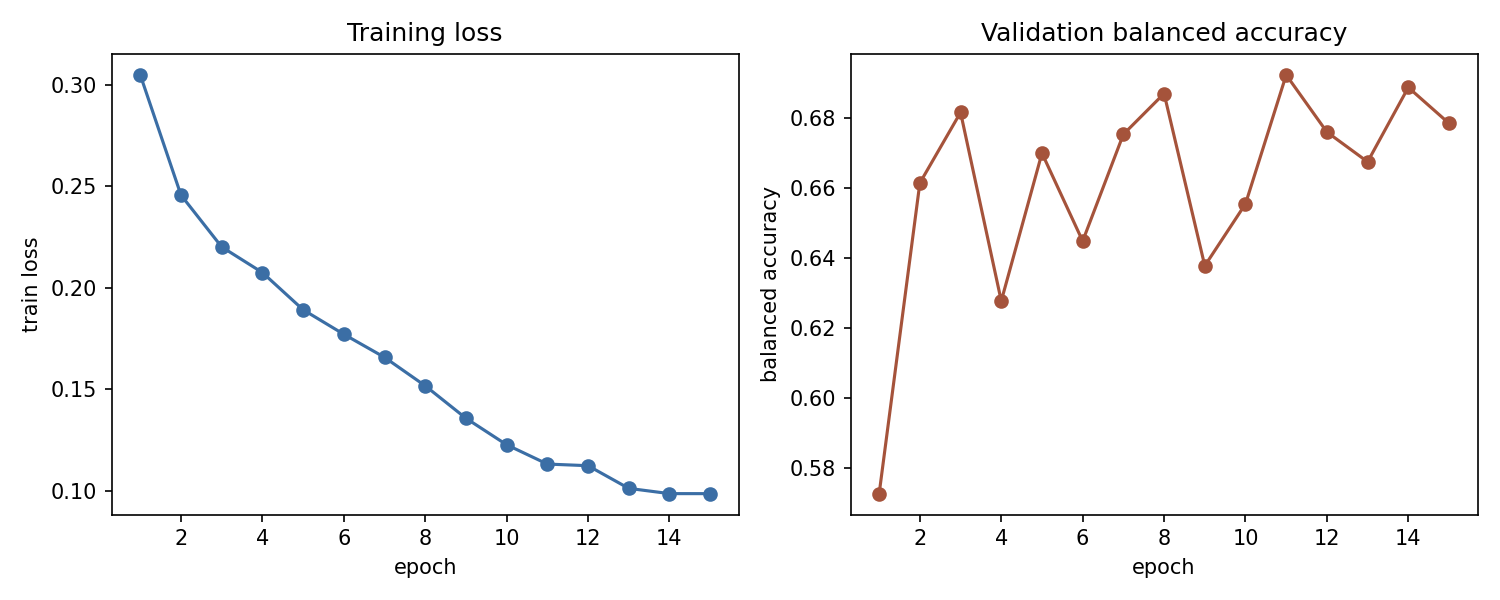
\includegraphics[width=\linewidth]{stage2_best_sensitivity_training_curves.png}
  \caption{Training loss and validation balanced accuracy for the median seed of ResNet-50 with the CE baseline. The model trains for 15 epochs and restores the best validation checkpoint.}
  \label{fig:training}
\end{figure}

\begin{figure}[t]
  \centering
  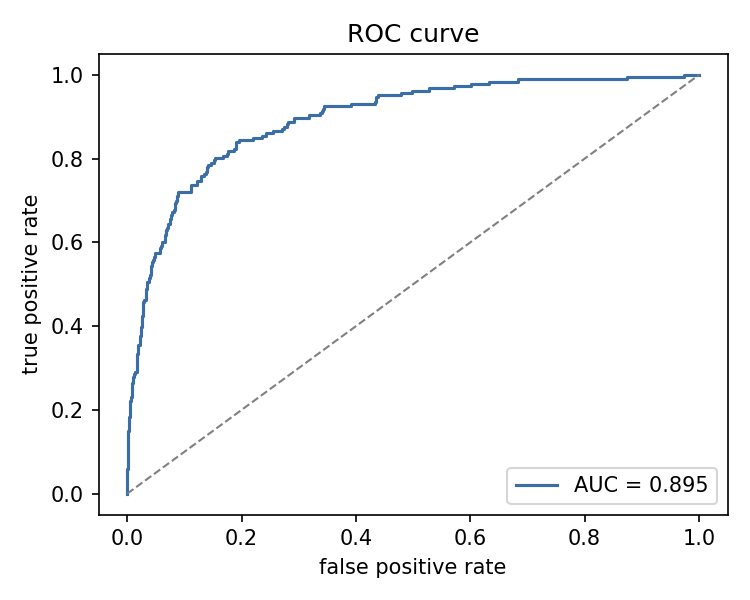
\includegraphics[width=0.72\linewidth]{stage2_best_sensitivity_roc_test.png}
  \caption{Test ROC curve for the median seed of ResNet-50 with the CE baseline. The operating threshold is selected on validation at 95\% specificity.}
  \label{fig:roc}
\end{figure}
